% l = 8
\mbox{}\\[-0.75in]
\begin{figure}[!b]
\begin{center}
\subfloat{
\resizebox{8cm}{4.5cm}{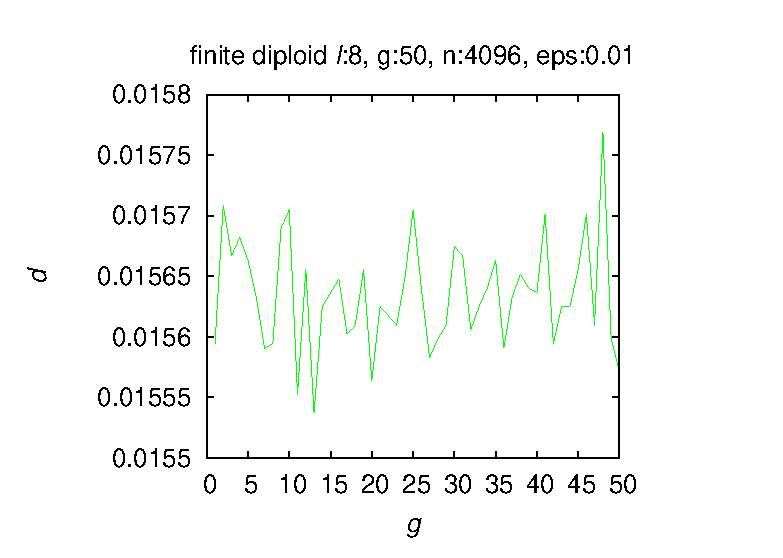
\includegraphics{figures/eps/vio/mu/b8/e0.01/n00004096_fin_dip.eps}}}\hspace{-3em}%
\subfloat{
\resizebox{8cm}{4.5cm}{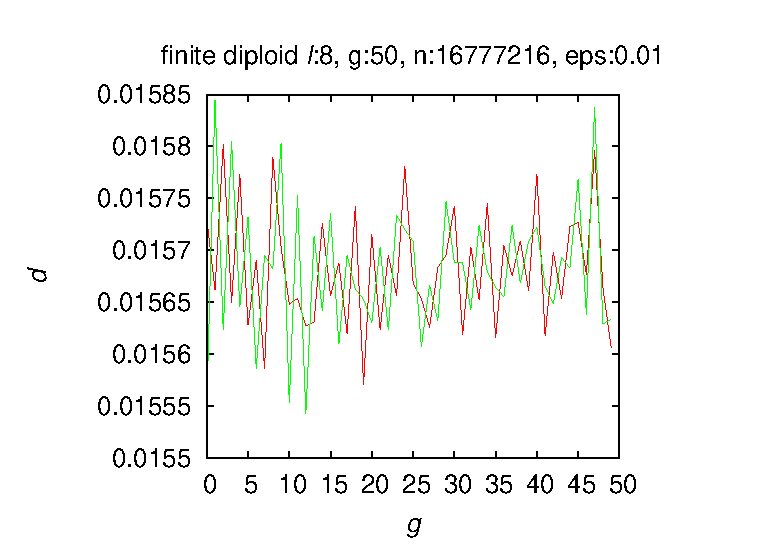
\includegraphics{figures/eps/vio/mu/b8/e0.01/n00004096_fin_dip_wovio.eps}}}\vspace{-1em}  \hspace{-3em}%
\end{center}
\begin{center}
\subfloat{
\resizebox{8cm}{4.5cm}{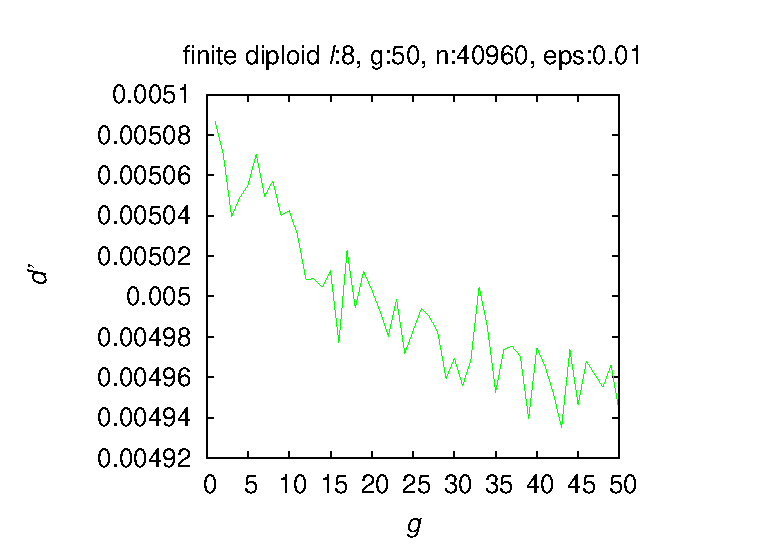
\includegraphics{figures/eps/vio/mu/b8/e0.01/n00040960_fin_dip.eps}}}\hspace{-3em}%
\subfloat{
\resizebox{8cm}{4.5cm}{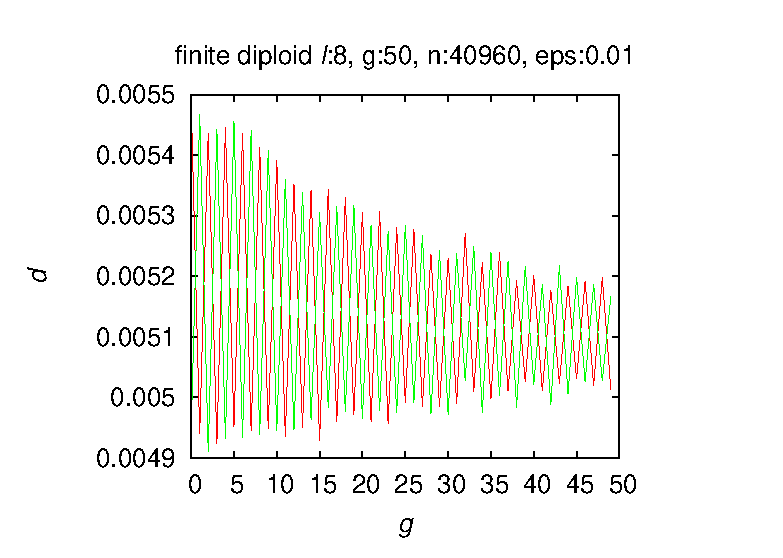
\includegraphics{figures/eps/vio/mu/b8/e0.01/n00040960_fin_dip_wovio.eps}}}\vspace{-1em}  \hspace{-3em}%
\end{center}

\begin{center}
\subfloat{
\resizebox{8cm}{4.5cm}{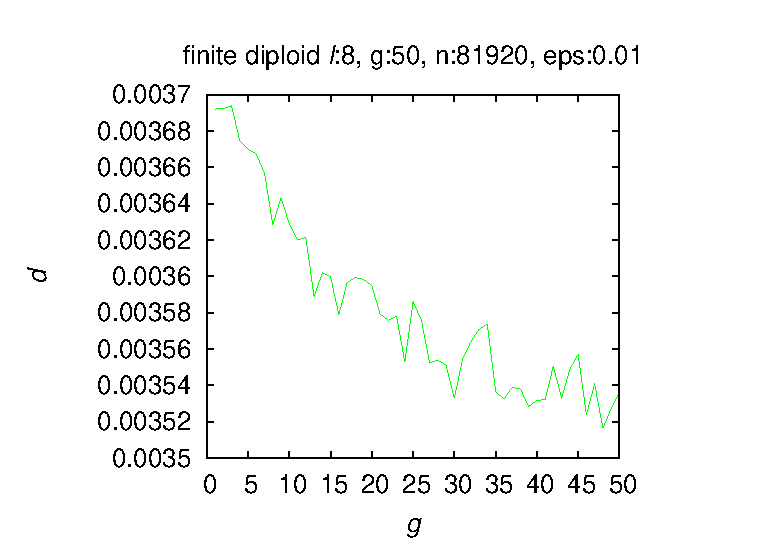
\includegraphics{figures/eps/vio/mu/b8/e0.01/n00081920_fin_dip.eps}}}\hspace{-3em}%
\subfloat{
\resizebox{8cm}{4.5cm}{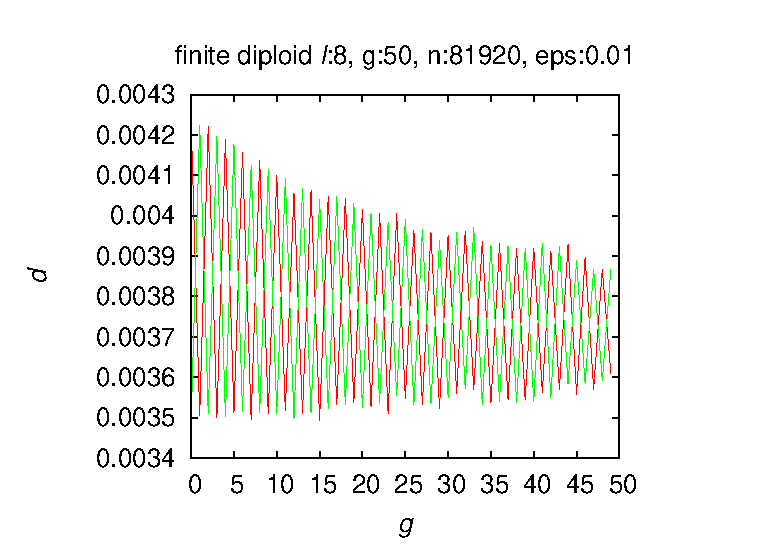
\includegraphics{figures/eps/vio/mu/b8/e0.01/n00081920_fin_dip_wovio.eps}}}\vspace{-1em}  \hspace{-3em}%
\end{center}

\begin{center}
\subfloat{
\resizebox{8cm}{4.5cm}{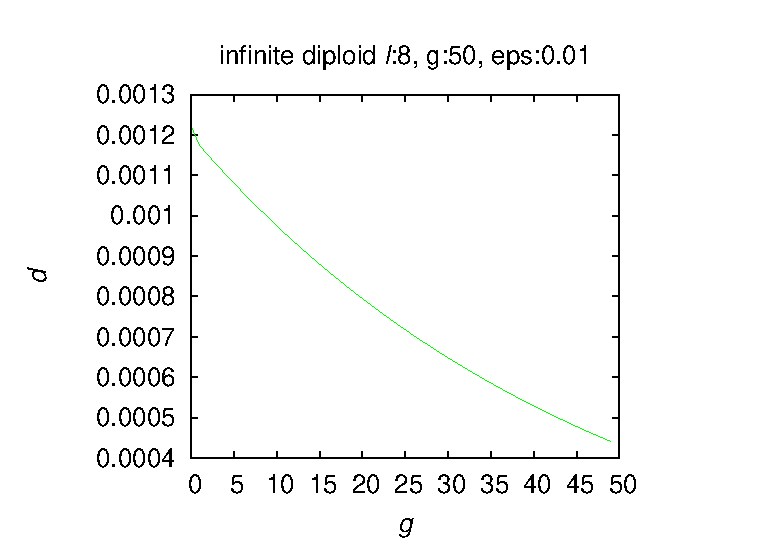
\includegraphics{figures/eps/vio/mu/b8/e0.01/inf_dip.eps}}}\hspace{-3em}%
\subfloat{
\resizebox{8cm}{4.5cm}{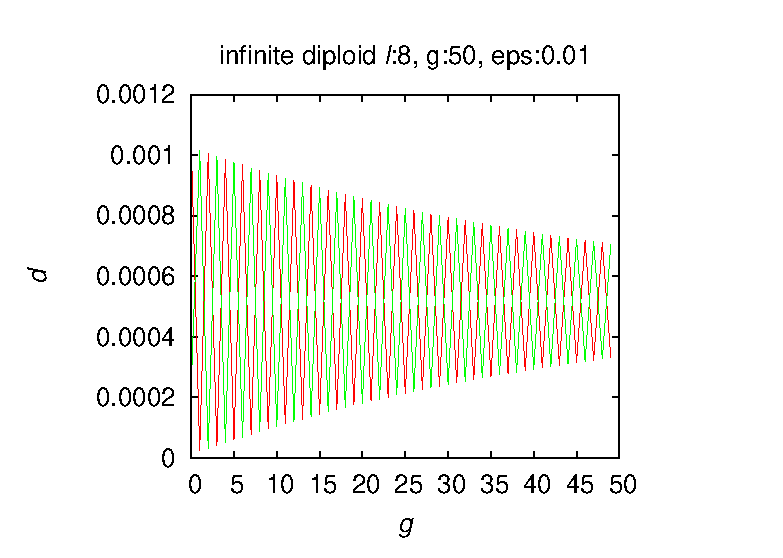
\includegraphics{figures/eps/vio/mu/b8/e0.01/inf_dip_wovio.eps}}}\vspace{-0.5em}  \hspace{-3em}%


\caption[\textbf{Infinite and finite diploid population oscillation behavior in case of violation in $\bm{\mu}$ for genome length $\ell = 8$ and $\bm{\epsilon} = 0.01$}]
{\textbf{Infinite and finite diploid population behavior for $\bm{\mu}$ violation, $\ell = 8$ and $\bm{\epsilon} = 0.01$:} 
  In left column, $d'$ is distance of finite population or infinite population to limit $\bm{z}^\ast$ for $g$ generations. 
  In right column, $d$ is distance of finite population or infinite population to limits $\bm{p}^\ast$ and $\bm{q}^\ast$.}
\label{oscillation_8d_vio_mu_0.01}
\end{center}
\end{figure}

% l = 10

\begin{figure}[h]
\begin{center}
\subfloat{
\resizebox{8cm}{4.5cm}{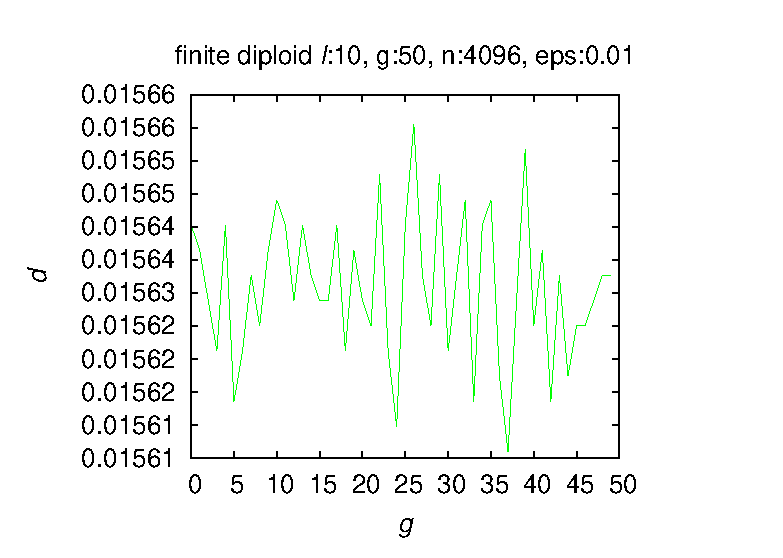
\includegraphics{figures/eps/vio/mu/b10/e0.01/n00004096_fin_dip.eps}}}\hspace{-3em}%
\subfloat{
\resizebox{8cm}{4.5cm}{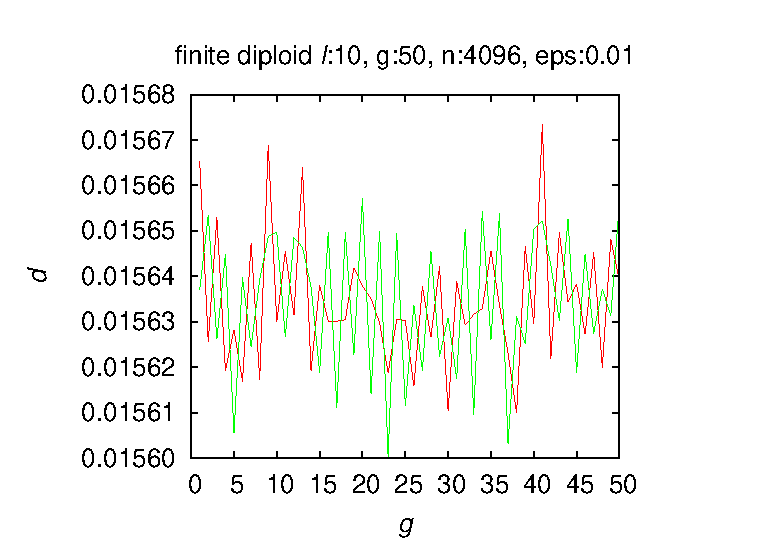
\includegraphics{figures/eps/vio/mu/b10/e0.01/n00004096_fin_dip_wovio.eps}}}\vspace{-1em}  \hspace{-3em}%
\end{center}
\begin{center}
\subfloat{
\resizebox{8cm}{4.5cm}{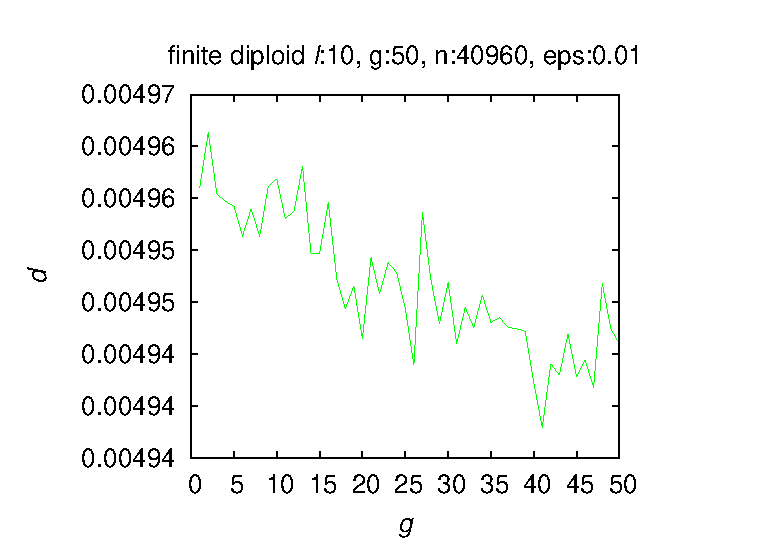
\includegraphics{figures/eps/vio/mu/b10/e0.01/n00040960_fin_dip.eps}}}\hspace{-3em}%
\subfloat{
\resizebox{8cm}{4.5cm}{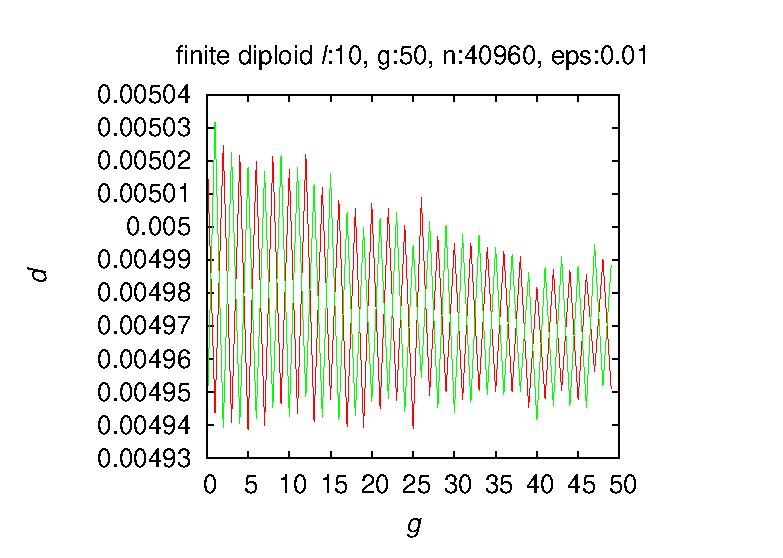
\includegraphics{figures/eps/vio/mu/b10/e0.01/n00040960_fin_dip_wovio.eps}}}\vspace{-1em}  \hspace{-3em}%
\end{center}


\begin{center}
\subfloat{
\resizebox{8cm}{4.5cm}{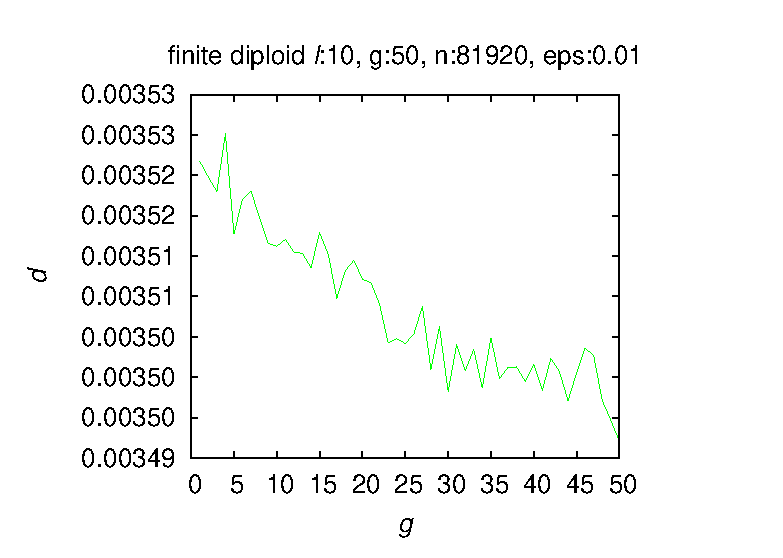
\includegraphics{figures/eps/vio/mu/b10/e0.01/n00081920_fin_dip.eps}}}\hspace{-3em}%
\subfloat{
\resizebox{8cm}{4.5cm}{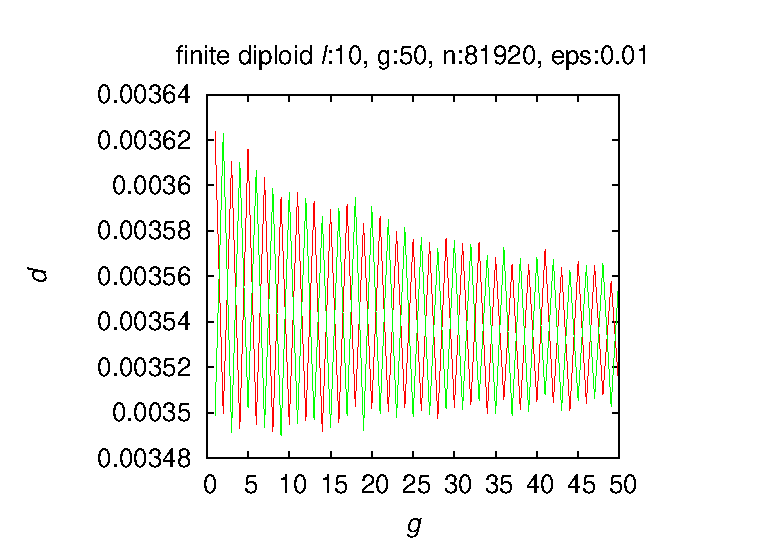
\includegraphics{figures/eps/vio/mu/b10/e0.01/n00081920_fin_dip_wovio.eps}}}\vspace{-1em}  \hspace{-3em}%
\end{center}

\begin{center}
\subfloat{
\resizebox{8cm}{4.5cm}{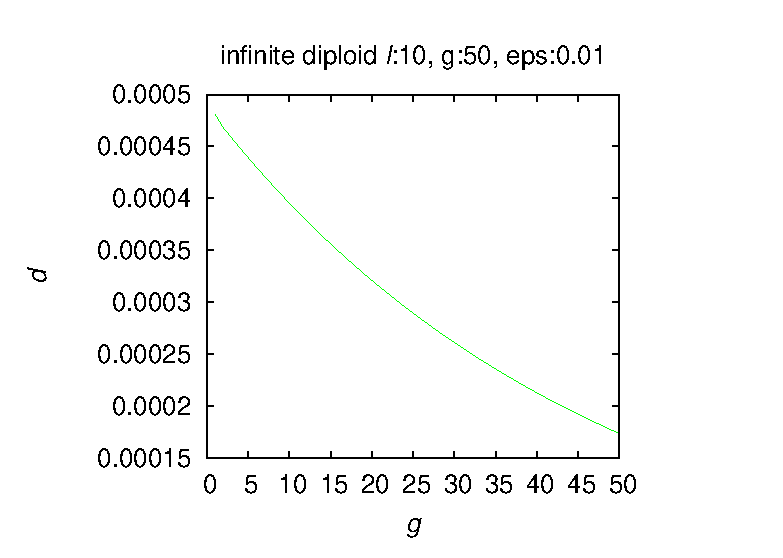
\includegraphics{figures/eps/vio/mu/b10/e0.01/inf_dip.eps}}}\hspace{-3em}%
\subfloat{
\resizebox{8cm}{4.5cm}{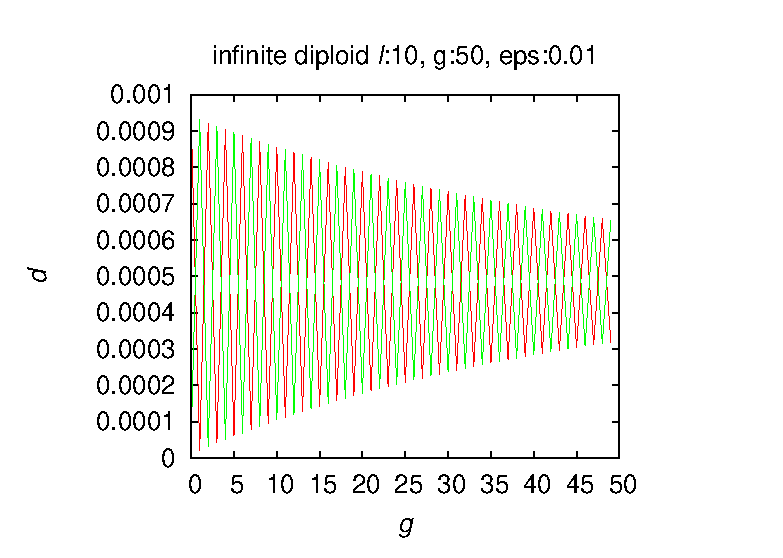
\includegraphics{figures/eps/vio/mu/b10/e0.01/inf_dip_wovio.eps}}}\vspace{-0.5em}  \hspace{-3em}%


\caption[\textbf{Infinite and finite diploid population oscillation behavior in case of violation in $\bm{\mu}$ for genome length $\ell = 10$ and $\bm{\epsilon} = 0.01$}]{\textbf{Infinite and finite diploid population oscillation behavior in case of violation in $\bm{\mu}$ for genome length $\ell = 10$ and $\bm{\epsilon} = 0.01$:} 
  In left column, $d'$ is distance of finite population of size $n$ or infinite population to limit $\bm{z}^\ast$ for $g$ generations. In right column, $d$ is distance of finite population or infinite population to limits $\bm{p}^\ast$ and $\bm{q}^\ast$ without violation.}
\label{oscillation_10d_vio_mu_0.01}
\end{center}
\end{figure}

% l = 12

\begin{figure}[h]
\begin{center}
\subfloat{
\resizebox{8cm}{4.5cm}{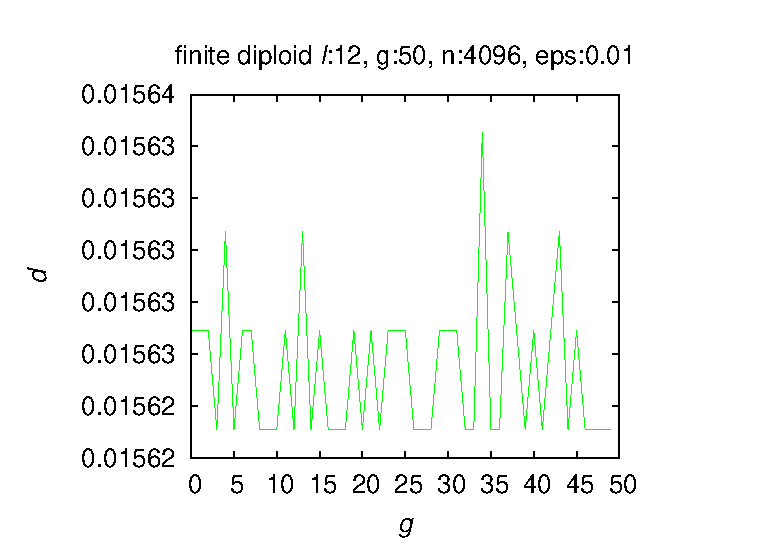
\includegraphics{figures/eps/vio/mu/b12/e0.01/n00004096_fin_dip.eps}}}\hspace{-3em}%
\subfloat{
\resizebox{8cm}{4.5cm}{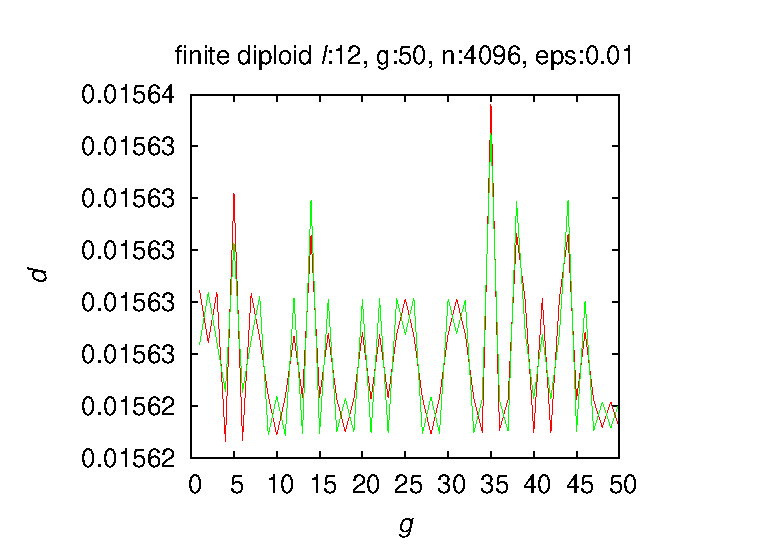
\includegraphics{figures/eps/vio/mu/b12/e0.01/n00004096_fin_dip_wovio.eps}}}\vspace{-1em}  \hspace{-3em}%
\end{center}
\begin{center}
\subfloat{
\resizebox{8cm}{4.5cm}{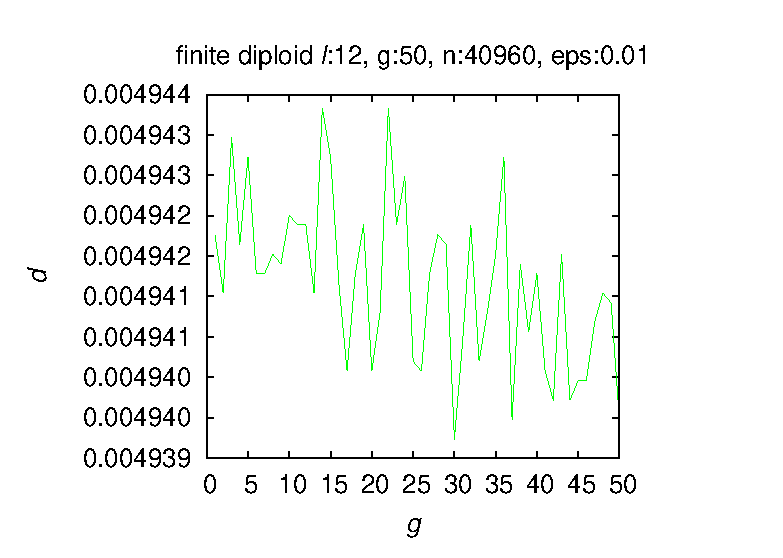
\includegraphics{figures/eps/vio/mu/b12/e0.01/n00040960_fin_dip.eps}}}\hspace{-3em}%
\subfloat{
\resizebox{8cm}{4.5cm}{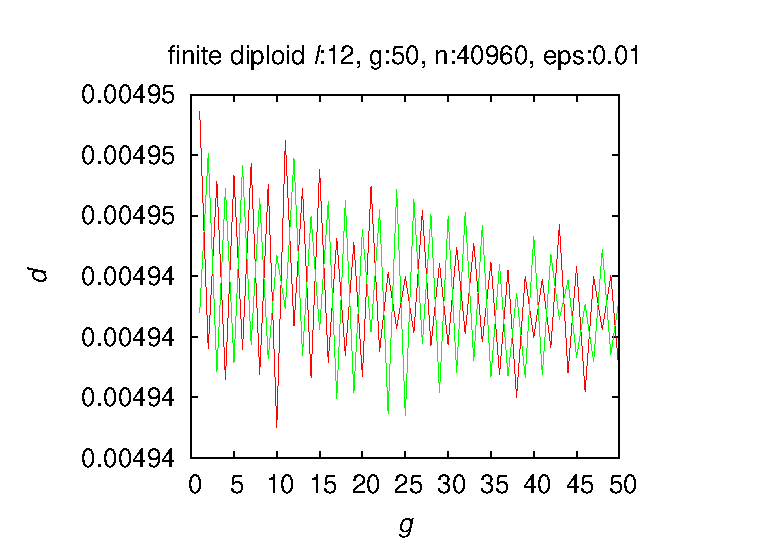
\includegraphics{figures/eps/vio/mu/b12/e0.01/n00040960_fin_dip_wovio.eps}}}\vspace{-1em}  \hspace{-3em}%
\end{center}


\begin{center}
\subfloat{
\resizebox{8cm}{4.5cm}{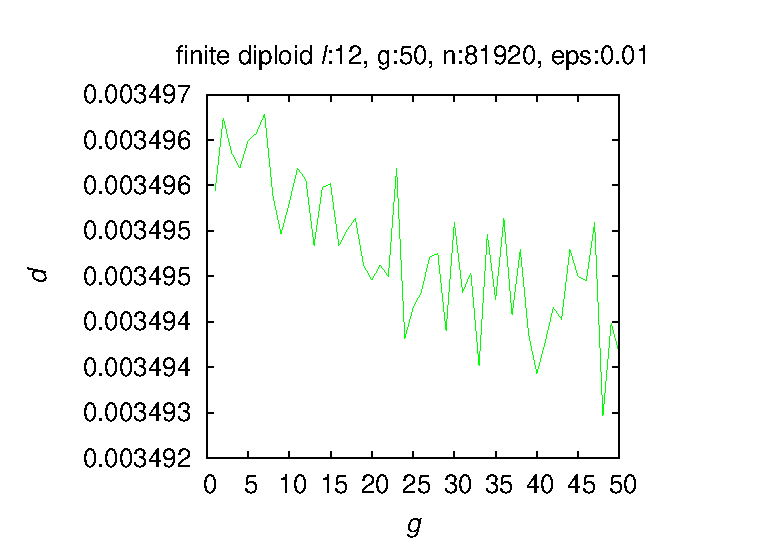
\includegraphics{figures/eps/vio/mu/b12/e0.01/n00081920_fin_dip.eps}}}\hspace{-3em}%
\subfloat{
\resizebox{8cm}{4.5cm}{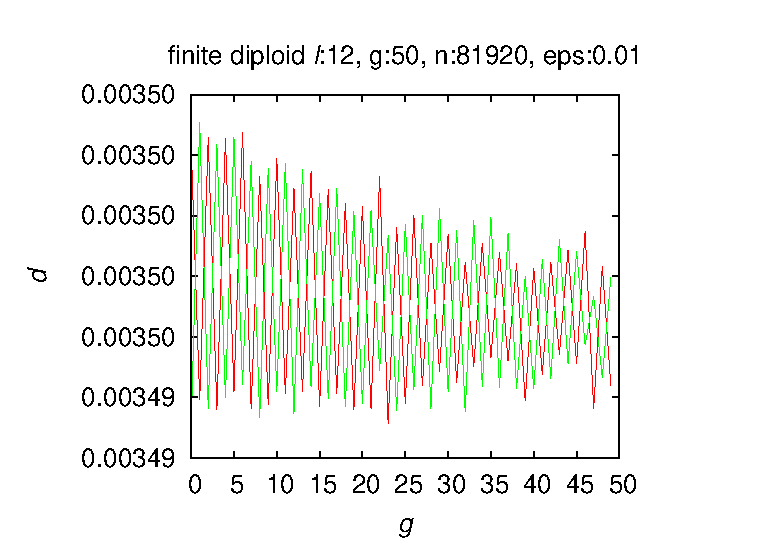
\includegraphics{figures/eps/vio/mu/b12/e0.01/n00081920_fin_dip_wovio.eps}}}\vspace{-1em}  \hspace{-3em}%
\end{center}

\begin{center}
\subfloat{
\resizebox{8cm}{4.5cm}{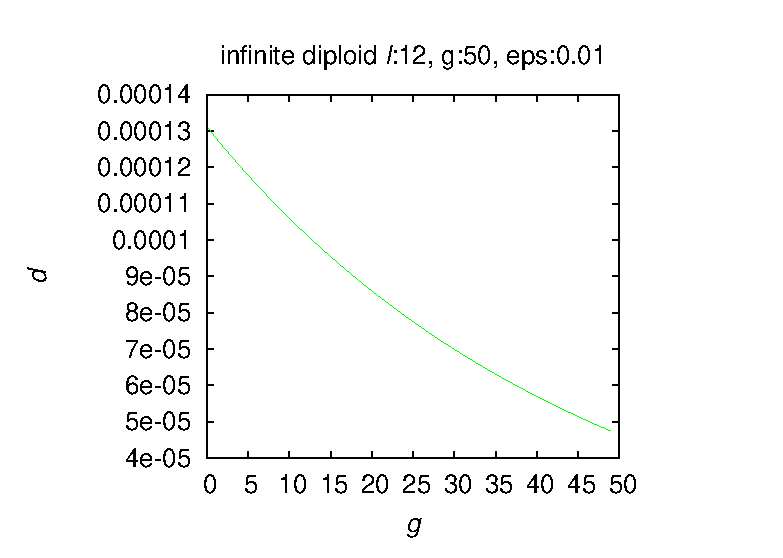
\includegraphics{figures/eps/vio/mu/b12/e0.01/inf_dip.eps}}}\hspace{-3em}%
\subfloat{
\resizebox{8cm}{4.5cm}{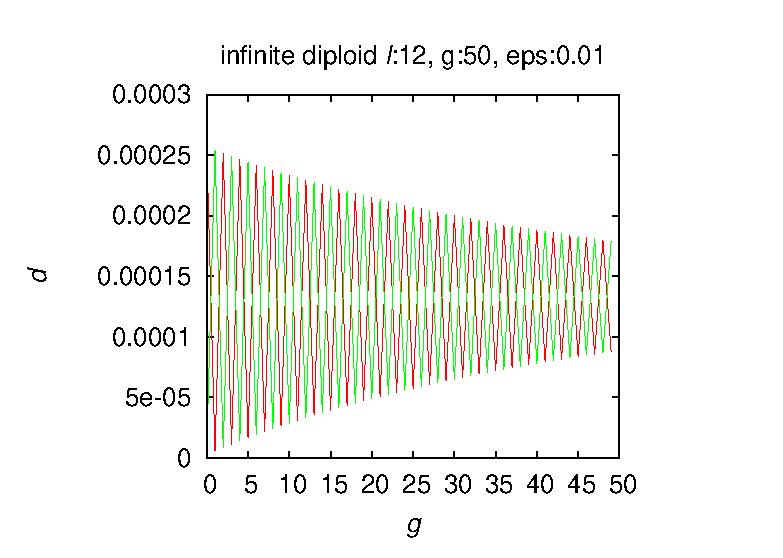
\includegraphics{figures/eps/vio/mu/b12/e0.01/inf_dip_wovio.eps}}}\vspace{-0.5em}  \hspace{-3em}%


\caption[\textbf{Infinite and finite diploid population oscillation behavior in case of violation in $\bm{\mu}$ for genome length $\ell = 12$ and $\bm{\epsilon} = 0.01$}]{\textbf{Infinite and finite diploid population oscillation behavior in case of violation in $\bm{\mu}$ for genome length $\ell = 12$ and $\bm{\epsilon} = 0.01$:} 
  In left column, $d'$ is distance of finite population of size $n$ or infinite population to limit $\bm{z}^\ast$ for $g$ generations. In right column, $d$ is distance of finite population or infinite population to limits $\bm{p}^\ast$ and $\bm{q}^\ast$ without violation.}
\label{oscillation_12d_vio_mu_0.01}
\end{center}
\end{figure}

% l = 14

\begin{figure}[h]
\begin{center}
\subfloat{
\resizebox{8cm}{4.5cm}{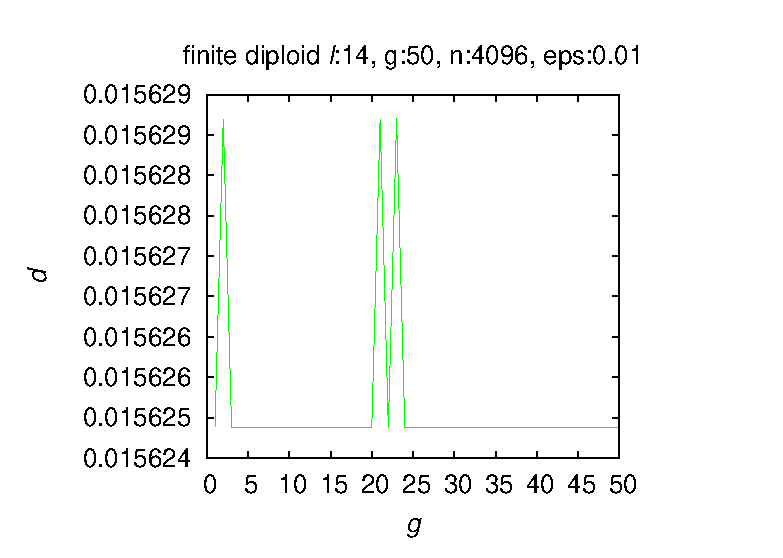
\includegraphics{figures/eps/vio/mu/b14/e0.01/n00004096_fin_dip.eps}}}\hspace{-3em}%
\subfloat{
\resizebox{8cm}{4.5cm}{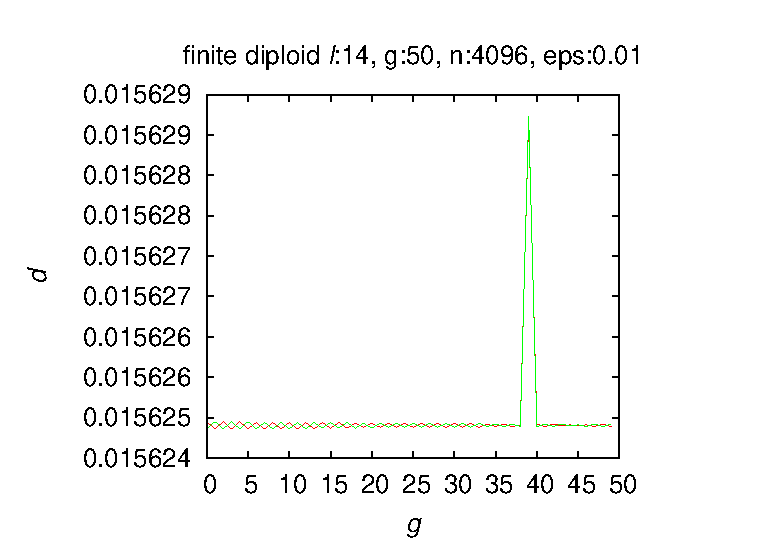
\includegraphics{figures/eps/vio/mu/b14/e0.01/n00004096_fin_dip_wovio.eps}}}\vspace{-1em}  \hspace{-3em}%
\end{center}
\begin{center}
\subfloat{
\resizebox{8cm}{4.5cm}{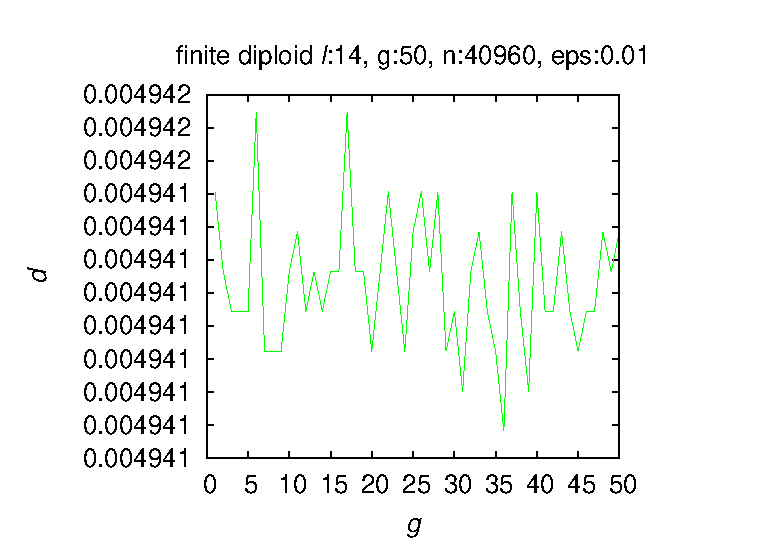
\includegraphics{figures/eps/vio/mu/b14/e0.01/n00040960_fin_dip.eps}}}\hspace{-3em}%
\subfloat{
\resizebox{8cm}{4.5cm}{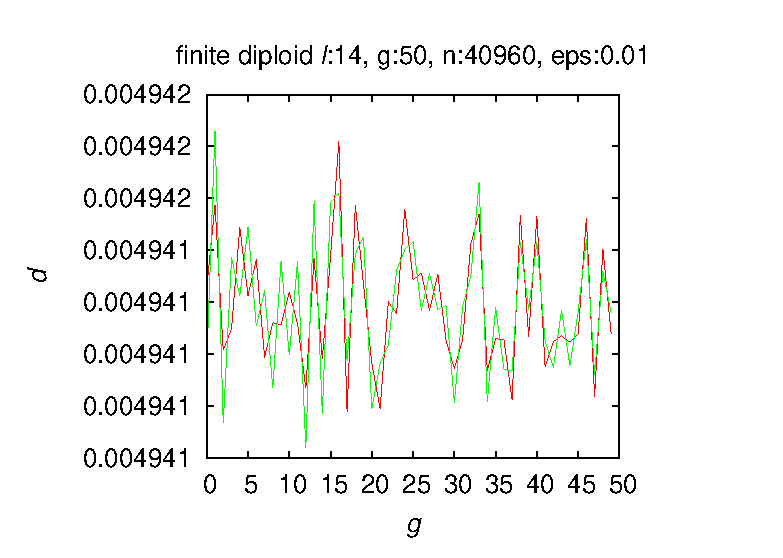
\includegraphics{figures/eps/vio/mu/b14/e0.01/n00040960_fin_dip_wovio.eps}}}\vspace{-1em}  \hspace{-3em}%
\end{center}


\begin{center}
\subfloat{
\resizebox{8cm}{4.5cm}{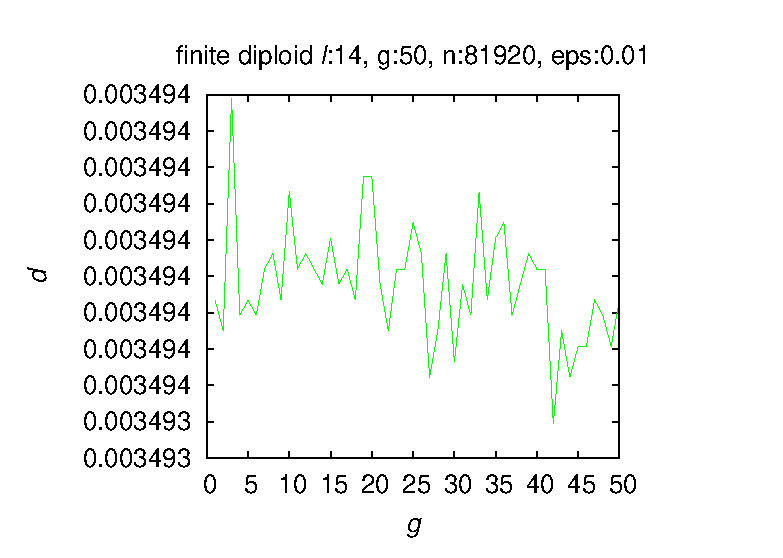
\includegraphics{figures/eps/vio/mu/b14/e0.01/n00081920_fin_dip.eps}}}\hspace{-3em}%
\subfloat{
\resizebox{8cm}{4.5cm}{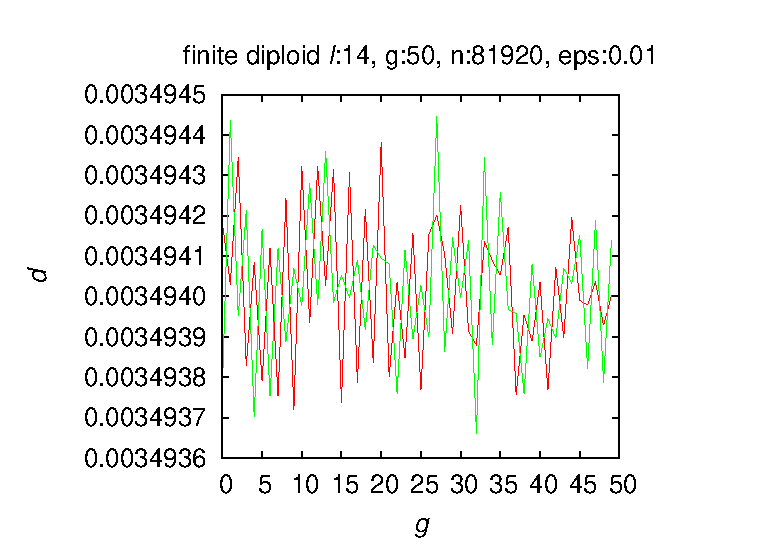
\includegraphics{figures/eps/vio/mu/b14/e0.01/n00081920_fin_dip_wovio.eps}}}\vspace{-1em}  \hspace{-3em}%
\end{center}

\begin{center}
\subfloat{
\resizebox{8cm}{4.5cm}{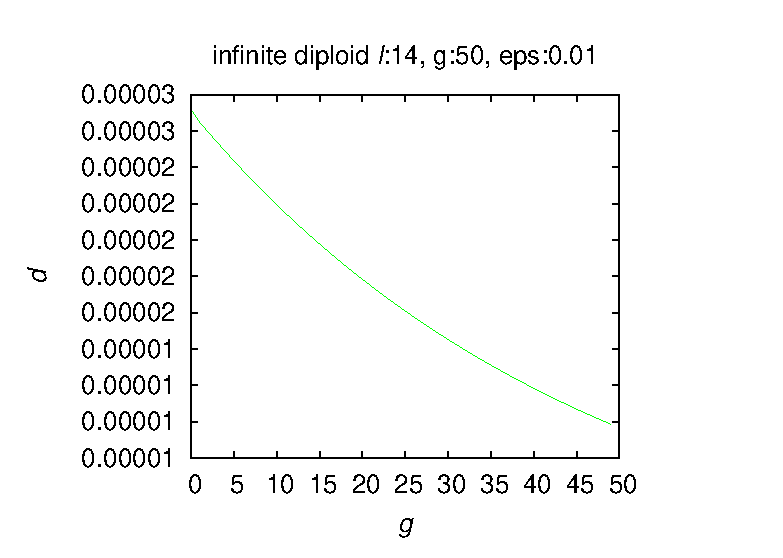
\includegraphics{figures/eps/vio/mu/b14/e0.01/inf_dip.eps}}}\hspace{-3em}%
\subfloat{
\resizebox{8cm}{4.5cm}{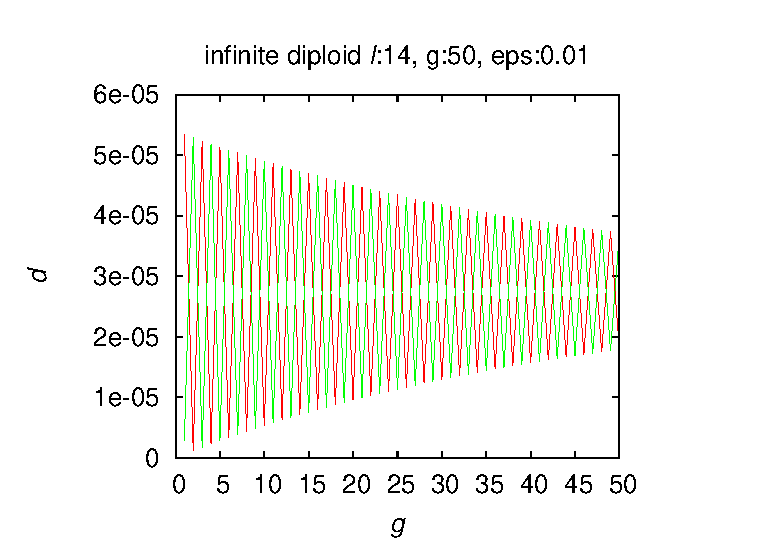
\includegraphics{figures/eps/vio/mu/b14/e0.01/inf_dip_wovio.eps}}}\vspace{-0.5em}  \hspace{-3em}%


\caption[\textbf{Infinite and finite diploid population oscillation behavior in case of violation in $\bm{\mu}$ for genome length $\ell = 14$ and $\bm{\epsilon} = 0.01$}]{\textbf{Infinite and finite diploid population oscillation behavior in case of violation in $\bm{\mu}$ for genome length $\ell = 14$ and $\bm{\epsilon} = 0.01$:} 
  In left column, $d'$ is distance of finite population of size $n$ or infinite population to limit $\bm{z}^\ast$ for $g$ generations. In right column, $d$ is distance of finite population or infinite population to limits $\bm{p}^\ast$ and $\bm{q}^\ast$ without violation.}
\label{oscillation_14d_vio_mu_0.01}
\end{center}
\end{figure}

\clearpage
The right column in figures \ref{oscillation_8d_vio_mu_0.01} through \ref{oscillation_14d_vio_mu_0.01} 
shows distance of finite and infinite diploid populations to non-violation limits $\bm{p^\ast}$ and $\bm{q^\ast}$ with $\bm{\epsilon} \;=\; 0.01$. 
Those graphs indicate oscillating behavior of diploid population given violation. 
Both finite and infinite populations oscillate given violation. Since the value of $\bm{\epsilon}$ 
is very small, damping of ripples is slow. The all zeros mask created in mutation distribution with $\bm{\epsilon} \;=\; 0.01$ has small 
probability of being used during mutation. Infinite population oscillation does not die out in 50 generations but will eventually die out. 
Even though oscillation in finite population is tapering down,
will not die out completely; because the Markov chain is regular, 
oscillation must reappear infinitely often.

The left column of figures \ref{oscillation_8d_vio_mu_0.01} through \ref{oscillation_14d_vio_mu_0.01} 
shows distance of finite and infinite diploid populations to limit $\bm{z^\ast}$ 
(limit with violation in mutation distribution $\bm{\mu}$) when $\bm{\epsilon} \;=\; 0.01$. 
The distance decreases as finite population size increases, 
and finite population shows behavior similar to infinite population as population size grows. 
Average distance data for diploid population for $\bm{\mu}$ violation 
with $\bm{\epsilon} \;=\; 0.01$ are tabulated in table \ref{distanceMuDipEps0.01}.

\begin{table}[h]
\caption[\textbf{Distance measured for violation in $\bm{\mu}$ with $\bm{\epsilon} \;=\; 0.01$ for diploids}]{\textbf{Distance measured for violation in $\bm{\mu}$ with $\bm{\epsilon} \;=\; 0.01$ for diploids:} $\ell$ is genome length, 
average distance between finite and infinite population is tabulated in the last three columns, and last row is expected single step distance.}
\centering
\begin{tabularx}{0.75\textwidth}{ c *{3}{X}}
\toprule
$\ell$ & $N = 4096$ & $N = 40960$ & $N = 81920$ \\
\midrule
8 & 0.0156	&  0.0050	& 0.0035 \\
10 & 0.0156	&  0.0049	& 0.0035 \\
12 & 0.0156	&  0.0049	& 0.0035 \\
14 & 0.0156	&  0.0049	& 0.0035 \\
\midrule
$1/\sqrt{N}$ & 0.0156 & 0.0049 & 0.0035 \\
\bottomrule
\end{tabularx}
\label{distanceMuDipEps0.01}
\end{table}
Table \ref{distanceMuDipEps0.01} shows that the average distance between 
finite population and infinite population decreases with increasing string length, a
pproaching the expected single step distance $1/\sqrt{N}$. 



